\chapter{Tecnologias Utilizadas}
    \section{Docker}
	\subsection{Breve história das tecnologias de contêineres}
	A história dos Contêineres começa em 1979 no Unix L7. Nele foi introduzido a chamada de sistema (\textit{system call}) \textit{chroot} capaz de mudar o diretório raiz de um processo e de seus processos filhos para um novo local no sistema de arquivos. Este avanço foi o início do conceito de isolamento de processos, pois limitava o acesso de cada processo ao sistema de arquivos. 

	Em 2000, surgiu o FreeBSD Jail, que permitia a administradores particionar um sistema FreeBSD em vários sistemas menores isolados e independentes, chamados de “\textit{jails}”. O sistema é similar ao \textit{chroot}, mas incluiu recursos de isolamento adicionais em diversos aspectos do sistema operacional, como por exemplo a atribuição de um endereço de IP diferente para cada \textit{jail}. \cite{abriefhistoryofcontainers}

	Em 2001, foi lançado o Linux VServer que, assim como o FreeBSD Jail, também é um mecanismo de \textit{jail} que pode particionar recursos (sistema de arquivos, endereços de rede, memória) em um sistema computacional. Isso é realizado por meio de níveis de isolamento do \textit{kernel}. Cada partição é chamada \textit{security context} e o sistema virtualizado dentro dele é chamado de \textit{virtual private server}. \cite{linuxvserver}

	Em 2004, foi lançado o Solaris Zones para sistemas x86 e SPARC. Cada \textit{zone} age como um servidor virtual completamente isolado dentro de uma única instância. Existem dois tipos de \textit{zones}: zonas globais (\textit{Global Zones}) e não-globais (\textit{Non-Global Zones}). A zona global é o ambiente de SO tradicional e é a área onde o SO Solaris está instalado. Todas as operações do sistema, como instalações, inicializações e desligamentos são feitas na zona global. As zonas não-globais, comumente chamadas somente de zonas, tem seus recurso e limites definidos pela zona global a que pertencem  \cite{introductiontosolariszone}

	Em 2005 a empresa Virtuozzo lançou o OpenVZ, que utiliza o \textit{kernel} do Linux para fornecer virtualização, isolamento, gerenciamento de recursos e \textit{checkpointing}. Cada contêiner OpenVZ possui um sistema de arquivos isolado, usuários e grupos de usuários, uma árvore de processos, rede, dispositivos e comunicação entre processos. Uma desvantagem da solução é que seu funcionamento depende da aplicação de um \textit{patch} no \textit{kernel} do Linux. \cite{openvz}

	Em 2006 engenheiros da Google desenvolveram o Process Containers, projetado para limitar, contabilizar e isolar o uso de recursos computacionais (CPU, memória, I/O do disco, rede) de uma coleção de processos. Um ano depois o projeto foi renomeado para Control Groups (\textit{cgroups}) e foi adicionado ao \textit{kernel} do Linux na versão \textit{2.6.24}.

	Em 2008 surgiu o LXC (LinuX Containers), que foi a primeira e mais completa implementação de um gerenciador de contêineres Linux. Foi implementado utilizando \textit{cgroups} e Linux \textit{namespaces} e funciona no \textit{kernel} do Linux sem a necessidade da aplicação de \textit{patches}.
	
	Em 2011 a empresa CloudFoundry iniciou o projeto Warden, que utilizava LXC em suas primeiras implementações, porém depois foi substituído por soluções próprias da empresa. Warden roda em formato \textit{daemon} e pode isolar ambientes em qualquer sistema operacional. Além disso, provê uma API para o gerenciamento de \textit{cgroups}, \textit{namespaces}, ciclo de vida dos processos e dos contêineres em diversos \textit{hosts} através de um modelo cliente-servidor.

	Finalmente, em 2013, surgiu o Docker. Neste momento contêineres cresceram muito em popularidade, juntamente com o Docker em si.
	Assim como o Warden, o Docker utilizou LXC em seus primeiros estágios mas logo trocou por uma solução própria para gerenciamento de contêineres: o \textit{libcontainer}.
	O Docker se destacou de seus concorrentes por oferecer um ecossistema completo para o gerenciamento de contêineres, que será detalhado mais adiante.
	
	\subsection{Contêineres e Máquinas virtuais}
	
	A virtualização é a tecnologia que permite a criação de diferentes ambientes computacionais, chamados de virtuais por simular a interface que é esperada por um sistema operacional.
	
	Um dos principais componentes da arquitetura é o \textit{Hypervisor}. Ele gerencia a distribuição dos recursos computacionais na máquina física (armazenamento, processamento e memória) entre as várias máquinas virtuais, além de fornecer um isolamento entre elas. Ele é um componente que fica entre o \textit{hardware} e a máquina virtual e é necessário para o processo de virtualização.
	Entre os gerenciadores de máquinas virtuais mais populares no mercado, pode-se citar VMWare vSphere, VirtualBox, Xen, Hyper-V e KVM.

	No baixo nível, um contêiner é apenas um conjunto de processos que são isolados do resto do sistema. No caso do Docker, os contêineres compartilham o \textit{kernel} do sistema operacional hospedeiro e, frequentemente, os binários e bibliotecas também. Todos os componentes compartilhados são \textit{read-only}. Este compartilhamento de componentes reduzem a necessidade de se replicar código do sistema operacional, e isso significa que um único servidor pode executar múltiplos contêineres com uma única instalação do sistema operacional.

	Diferentemente, uma máquina virtual é constituída do espaço de usuário juntamente com o espaço do \textit{kernel} de um sistema operacional e o \textit{hardware} é virtualizado. Cada máquina virtual tem um sistema operacional e suas aplicações e elas compartilham entre si o \textit{hardware} do computador hospedeiro.

	Ambas as tecnologias provém ambientes isolados para execução de aplicações e podem ser utilizadas para empacotar e distribuir \textit{software}.

	Dado o menor número de camadas entre a aplicação e o \textit{hardware},  os contêineres tendem a ser mais leves e mais rápidos, tornando-os mais práticos para os ciclos de desenvolvimento e implantação de serviços. Comparativamente, o tempo de inicialização de uma máquina virtual é muito maior do que a de um contêiner equivalente, além de o espaço ocupado em disco ser uma ordem de magnitude maior. \cite{whatsthediffvmvscontainers}
	
	\begin{figure}[htb]
		\caption{\label{fig_circulo}Diferenças entre VMs e Contêiners}
		\begin{center}
    		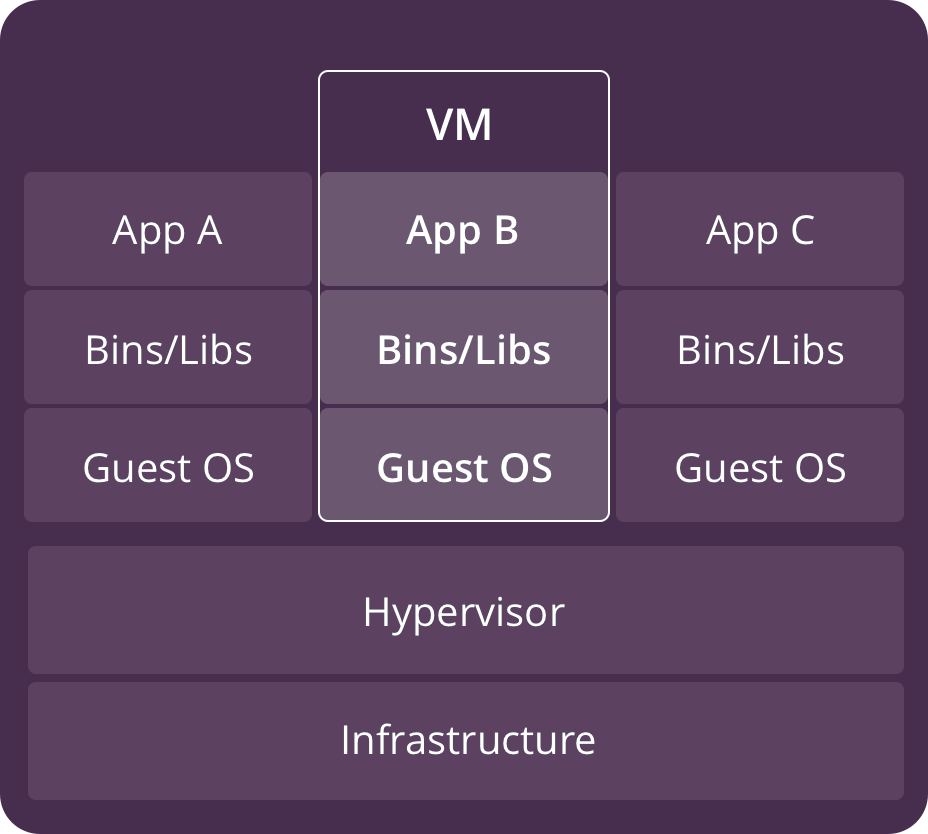
\includegraphics[scale=0.20]{pictures/vms.png}
    		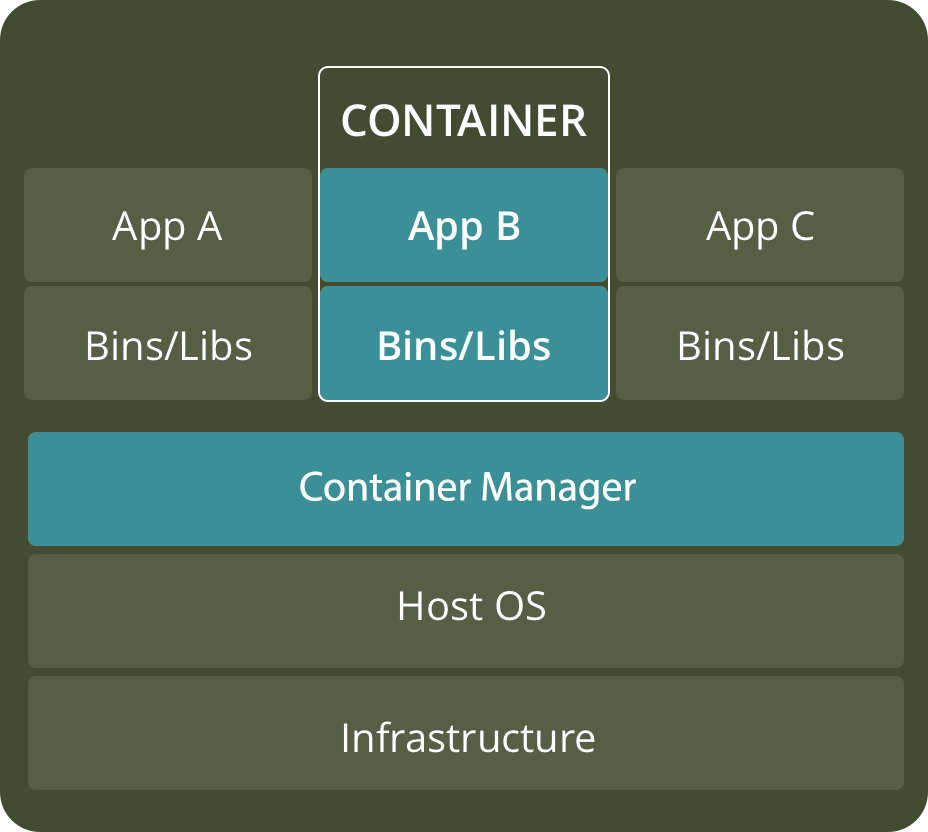
\includegraphics[scale=0.20]{pictures/containers.png}
		\end{center}
		\legend{Fonte: https://www.backblaze.com/blog/vm-vs-containers/}
	\end{figure}
	
	Ambos têm vantagens e desvantagens, e a decisão entre um outro varia dependendo dos casos de uso específicos, mas pode-se utilizar as seguintes regras como um ponto de partida:
	
	Máquinas virtuais são melhores para executar aplicações que necessitam de todos os recursos e funcionalidades do sistema operacional ou quando há uma variedade de sistemas operacionais para se gerenciar.
	
	Contêineres são uma escolha melhor quando a maior prioridade é maximizar o número de aplicações sendo executadas em um número mínimo de servidores.
	
	\section{Kubernetes}
	Kubernetes é um projeto de código aberto da Google, que possui mais de 1800 contribuintes e ganha cada vez mais atenção no mundo de operação e desenvolvimento de software. 
	O Google, dado a escala de sua operação, sofria com problemas com o gerenciamento de muitas máquinas virtuais. 
	Assim, o Google precisou repensar como lidar com esse problema, o que, depois de anos, levou ao gerenciador e escalonador de contêineres chamado Kubernetes.

	Para entender melhor a necessidade de um gerenciador tal como o Kubernetes, é necessário dar um passo atrás e olhar para as vantagens e desvantagens dos contêineres.
	Contêiners são feitos para serem leves, rápidos, mas de duração curta e frágeis.
	Assim, eles trocaram a resiliência de uma máquina virtual pela velocidade e leveza. Isso requer que contêineres rodem em um ambiente onde em caso de falha ou mudança de carga, esse ambiente garanta a substituição desses contêineres e gerencie eventuais mudanças de rede e recursos de memória do cluster.
	
    \section{GraphQL}
    GraphQL é uma linguagem de consulta criada pelo Facebook em 2002 e lançada publicamente em 2015. É utilizada principalmente em conjunto com o protocolo HTTP no contexto de um servidor web para que um cliente possa obter os dados que necessita de um servidor.
    Ele tem algumas características que torna seu uso interessante, como por exemplo:
    - Ela permite que o cliente especifique exatamente quais dados ele quer que sejam retornados em determinada requisição
    - Torna fácil o processo de agregação de dados vindos de diferentes fontes.
    - Utiliza um sistema de tipos para descrever dados.
    
    Além disso, a comunidade oferece diversos \textit{Frameworks} que atuam no lado do cliente e que são responsáveis pela obtenção, cacheamento e normalização dos dados. Os mais relevantes são Apollo e Relay (também desenvolvido e mantido pelo Facebook). Do lado do servidor, existe uma infinidade de implementações de GraphQL nas mais diferentes linguagens de programação, sendo a mais popular a implementação de referência em Javascript, mantida pela própria empresa criadora da linguagem.
    
    GraphQL é uma alternativa ao modelo REST e vem ganhando espaço no mercado nos últimos anos, sendo utilizado por grandes empresas como Facebook e Github em seus produtos mais importantes.
    
    
    
	\section{Clojure}
	
	Clojure é uma linguagem de programação dinâmica e funcional. Sendo um dialeto de LISP que roda na JVM, é uma linguagem compilada, mas que mantém todas características dinâmicas a ser utilizadas em Runtime. Possui compatibilidade e interoperabilidade com todo ecossistema Java e de outras linguagens que rodem na JVM. Clojure enfatiza o uso de estruturas de dados imutáveis e de a filosofia de Code is Data, com um sistema poderoso de macros e de estruturas de dados mutáveis Thread Safe quando necessário. \cite{clojurerationale}
	
	Clojure é a principal linguagem de programação utilizada no Nubank, e também é muito familiar para o grupo, além de apresentar características interessantes para o desenvolvimento do projeto. como a grande habilidade para lidar com problemas de concorrência de forma segura e eficiente.
	
	Dentro do desenvolvimento do projeto Clojure foi utilizada como uma das principais linguagens de programação para serviços de Backend. Um dos recursos que torna Clojure especialmente interessante é a possível interação em tempo real com o código através de um REPL (Read Eval Print Loop), algo que foi utilizado em um dos módulos do projeto como será descrito mais a frente. Além disso a familiaridade dos desenvolvedores do Nubank com a linguagem foi um fator decisivo para que o projeto pudesse continuar a ser mantido por mais pessoas no futuro.
	
	\begin{figure}
	    \centering
	    
\includegraphics[scale=0.1]{pictures/clojure_logo.png}
	    \caption{Logo Clojure}
	    \legend{Fonte: \url{https://cdn-images-1.medium.com/max/1200/1*eLqeIits5crU3G5b9LMEyg.png}}
	    \label{fig:logo_clojure}
	\end{figure}
	
	\section{Javascript} %% TODO: Paps
	Javascript é uma linguagem de programação interpretada baseada em ECMAScript. Foi originalmente criada para atuar junto com navegadores web, tornando possível que scripts fossem executados no lado do cliente sem passar pelo servidor, realizando comunicação assíncrona (AJAX) a manipulando o conteúdo do documento exibido em páginas web.
	Ela foi concebida par ser uma linguagem script com orientação a objetos baseada em protótipos, tipagem fraca de dinâmica e funções de primeira classe. Possui suporte à programação funcional e apresenta recursos como \textit{Closures} e \textit{higher-order functions}.
	
	Hoje é uma das linguagens mais populares do mundo e já há alguns anos vem sendo bastante utilizada no lado do servidor através de ambientes como Node.js. 
	
	
\subsection{Typescript}
Typescript é uma linguagem de programação desenvolvida e mantida pela Microsoft que tem como objetivo tornar bases de código em Javascript mais fáceis de se manter e menos suscetíveis à erros, através da adição de um sistema de tipos à linguagem, entre outros recursos. 

Para que o código escrito em Typescript possa de fato ser executado em ambientes como navegadores web e Node.js, é preciso compilá-lo para Javascript e este processo pode ser
feito através do compilador oferecido como parte do ferramental da linguagem. Na verdade, todo código Javascript é um código Typescript válido, porém o contrário não é verdadeiro.

\subsection{Node.js}
Node.js é um ambiente de execução multiplataforma e de código aberto, com a capacidade de executar Javascript fora do contexto de um browser, tornando possível o uso da linguagem em um ambiente de servidor.
Utiliza o motor de Javascript V8, desenvolvido pela Google e que está presente também em seu navegador Google Chrome. Node.js segue uma arquitetura \textit{event-driven} capaz de realizar I/O de maneira assíncrona e não bloqueante. Estas escolhas de projeto tem como objetivo otimizar o \textit{throughput} e escalabilidade em aplicações web com muitas operações de entrada e saída, bem como aplicações web \textit{real-time} como por exemplo programas de comunicação em tempo real e jogos.

Como parte de seu ecossistema, é oferecido um gerenciador de pacotes chamado \textit{npm}, que conta com uma interface de linha de comando e um banco de dados público de pacotes, que podem ser adicionados em projetos através de um sistema de dependência.

Hoje Node.js é utilizado por empresas como GoDaddy, Groupon, IBM, Linkedin, Microsoft, Netflix, PayPal, Rakuten, Walmart, Yahoo, entre outros.

\subsection{React}
React é uma biblioteca JavaScript de código aberto para criar interfaces interativas. É declarativa, eficiente e flexível e permite que o desenvolvedor componha interfaces complexas a partir de partes menores e isoladas chamadas "componentes".
Utiliza a técnica de \textit{Virtual DOM}, o que melhora drasticamente sua performance pois diminui o número de operações feitas de fato no DOM (\textit{Document Object Model}), que costumam ser tarefas de processamento mais intensivo.

\subsection{Electron}

	\section{ZeroMQ} %% TODO: Leo
	\section{Docker} %% TODO: Paps
	\section{Kubernetes} %% TODO: Leal
	